\section{Implementation}
We first started by benchmarking Distributed TF (using its \texttt{distributed\_replicated} mode), and Horovod. We used AWS p3.16xlarge instances for this, and found that Horovod scales as reported to 6k images per second at 64 GPUs (about 93 images per second per GPU). Distributed TF scaled to 6.5k images per second (about 100 images per second per GPU). Note that on a single node, both implementations can achieve around 200 images per second.

We started with the same ResNet101 model as used by the TF benchmarks, and verified that it could also achieve 200 images per second on a single node. The single node case can be understood as just the gradient and NCCL (intra-node) allreduce components seen in Figure \ref{fig:pipeline}. Our approach for the distributed setting was to use parameter server Ray actors to manage gradient aggregation between the Ray SGD actors that held the model replicas.

\begin{figure}
    \centering
    % 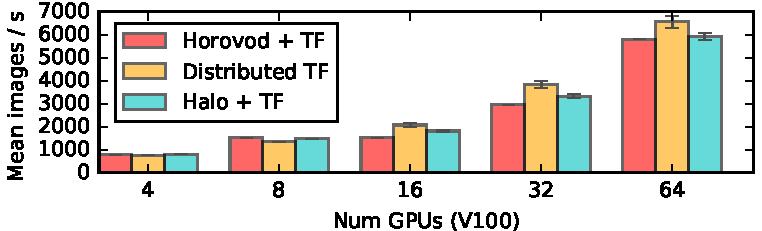
\includegraphics[width=3.1in,keepaspectratio]{fig/sgd_plot.pdf}
    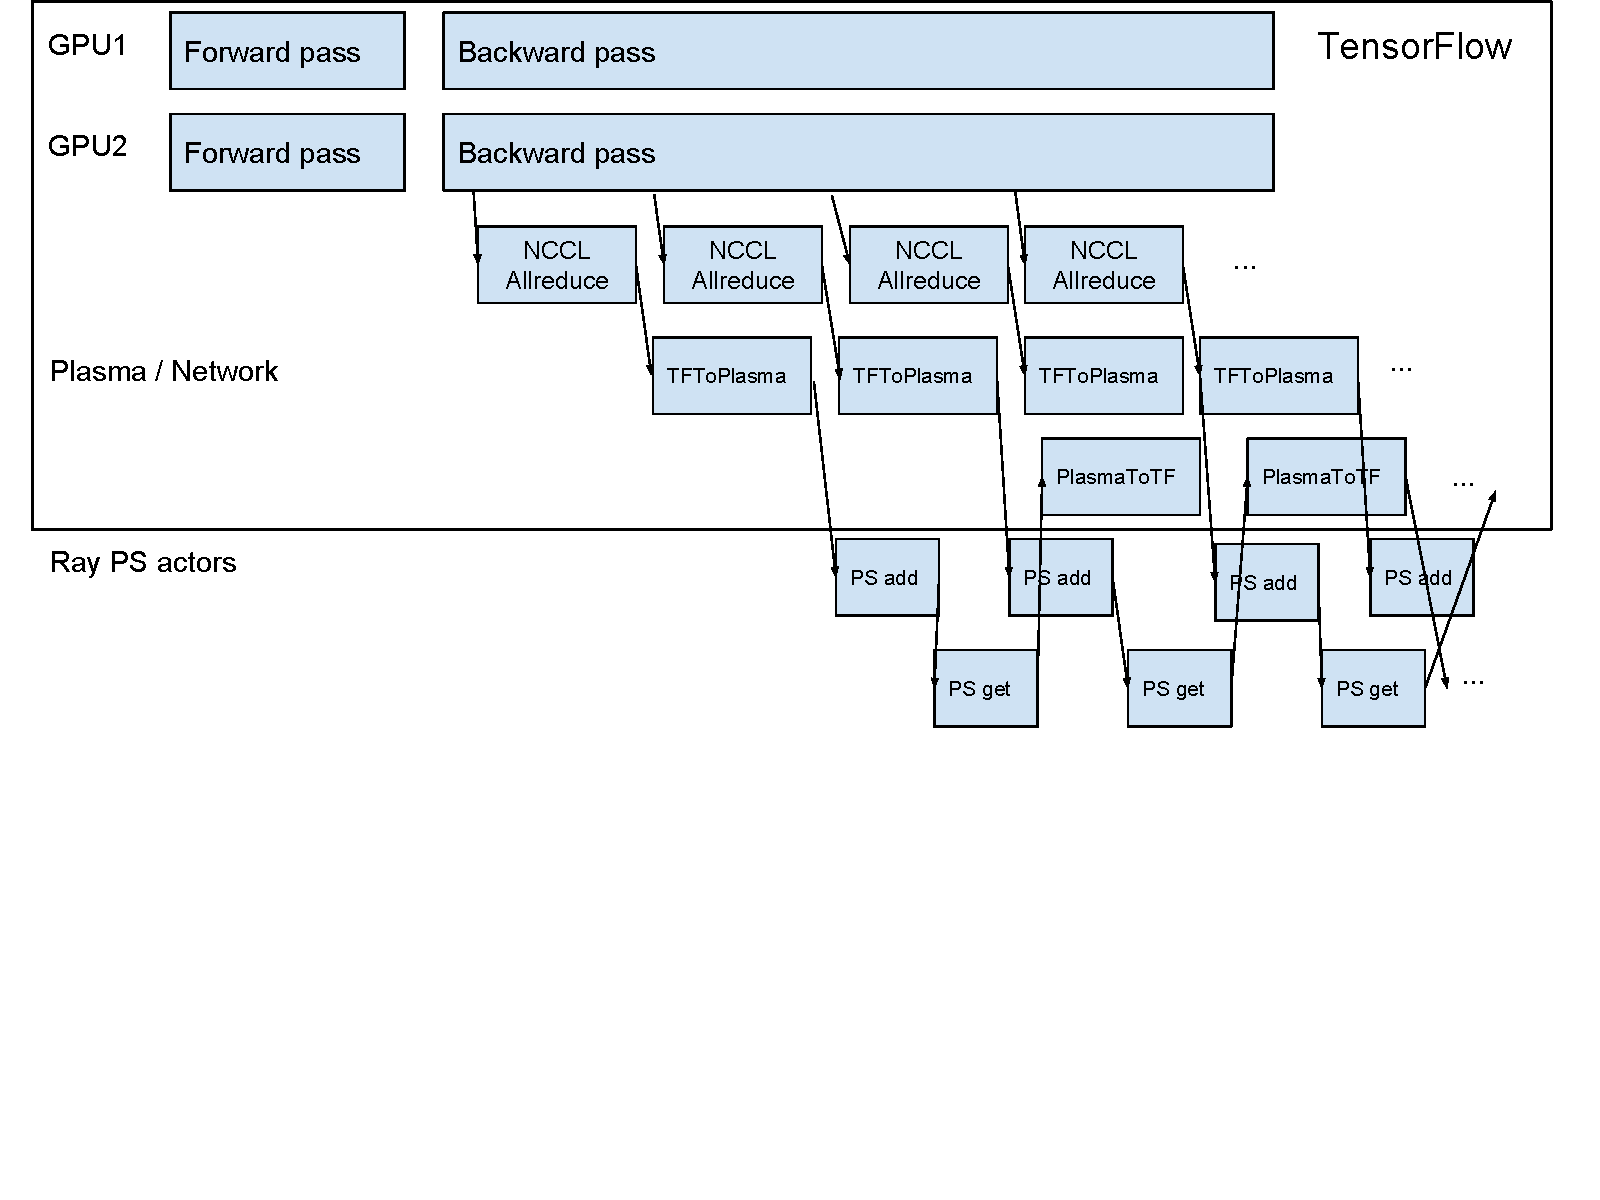
\includegraphics[width=5.1in,keepaspectratio]{fig/pipeline.pdf}
    \caption{
    \small{
        Timeline of our distributed SGD using a sharded parameter server implemented in Ray. The computation starts with the forward pass on GPUs. Gradients are produced by the backwards passed and averaged across GPUs via NCCL allreduce. As these intra-node allreduces finish, the averaged gradients are written to Ray's object store (TFToPlasma), where they are averaged across nodes by parameter server actors. The SGD actors then read back the averaged gradients from the parameter server actors (PlasmaToTF) and apply the gradients to their local model replica.
    }
    }
    \label{fig:pipeline}
\end{figure}

\subsection{Memory Transfer between TensorFlow and Ray}

In order to be achieve competitive levels of throughput, we had to utilize low-level primitives and write custom operators to avoid redundant copies and pipeline stages of the computation. All of our experiments used a Res-Net 101 model consisting of 168 MB of parameter weights. A standard forward pass with 64 images is roughly 40 ms.

The compute engine, TensorFlow, manages all tensor memory buffers within a node.  To communicate tensors (gradients, in the case of SGD) across nodes, we make use of Ray's \textit{distributed object store} component (named Plasma).  Hence, memory transfer must happen between TensorFlow and Ray.

The strawman approach is straightforward.  With \texttt{gradients = sess.run(compute\_op)}, one asks TensorFlow to run calculation and returns a newly allocated \texttt{numpy.ndarray} that resides on host memory.  Then, one could perform \texttt{object\_id = ray.put(gradients)}, which amounts to a host-to-host memory copy---from ndarray to Ray's object store.  The remote nodes can subsequently fetch this object via \texttt{ray.get(object\_id)}.  In total there are three copies: (1) device memory to host memory (\texttt{tf.Tensor} to \texttt{np.ndarray}), (2) host memory to host memory (ndarray to Ray's object store), then (3) across-node communication.

We improve upon the strawman by eliminating the three copies down to two, the minimum necessary amount, by circumventing numpy completely.  The approach is to insert two custom TensorFlow operators into the dataflow graph.  The \texttt{TensorToPlasma} op schedules \texttt{cudaMemcpy} directly from \texttt{tf.Tensor} device memory to Plasma host memory, eliminating the unnecessary \texttt{np.ndarray} buffer.  The \texttt{PlasmaToTensor} op assumes the reversed role, copying from Plasma host memory into TensorFlow on-device buffers.

To avoid stalling TensorFlow's compute, both ops create their own CUDA streams and launch the copy kernels onto their respective streams.  The host memory buffers are allocated and owned by Plasma, hence care has been taken to call CUDA's \texttt{cuMemHostRegister()} on those source/destination buffers; without such explicit registration, we observed that our custom copy ops stall the main compute stream, due to CUDA's ``default stream semantics''.  Lastly, to adhere to TensorFlow's dataflow semantics, care is taken to have our own copy streams properly synchronize on TensorFlow's compute stream, which makes sure any Tensor to copy has indeed been filled in by its upstream producer.

The above discussion assumes Tensor buffers reside on GPUs.  For CPU-owned Tensors, the strategy is to launch several threads that perform \texttt{memcpy()} on equal-sized chunks.  We note that this is a niche use case for deep learning users.

\subsection{Pipelining Computation with Communication}

We emphasize that, the above pipelining optimization is performed at the Ray level---that is, using Ray async actor method calls in the standard Ray programming model.  TensorFlow, the compute engine that launches CUDA kernels onto the GPUs, has implemented such pipelining at the device level.  Specifically, it uses at least 3 CUDA streams to dispatch kernels: a main stream for compute, a host-to-device copy stream, and a device-to-host copy stream.  Therefore, within a device, the communication and computation are already pipelined (up to black-box constraints imposed by the hardware).


As seen the above Figure~\ref{fig:pipeline}, all cross network pipelining of computation is handled outside TensorFlow.

\subsection{Gradient packing}
One key ingredient in enabling high performance was packing gradients. Gradient packing occurs after gradient calculation begins, and merges different size arrays from different layers into larger contiguous chunks. These chunks would later on be deconstructed back into the original tensor shapes in order to be applied to the model weights.

This enabled a couple different minor optimizations. First, it amortized the memory transfer overhead from GPU to Ray's shared memory object store, maximizing throughput. It also was necessary to efficiently saturate the network. On the other hand, the size of the gradient packed could not be too large, as the receiving node would oversaturate, causing an overall slower implementation. In our experiments, we pack into roughly 11MB chunks, resulting in 15 chunks.

\subsection{Parameter Server Sharding and Placement}
Instead of using a centralized parameter server, we would shard the original model weights into distinct sections. The placement of these shards was important, as misplacement could reduce bandwidth. In our implementation, we make sure all parameter server shards are evenly placed on the nodes in a round-robin fashion.

\subsection{Scalability Bottlenecks}
\subsubsection{Network Bandwidth}
With all implementations, throughput dropped nearly 2x when going from one machine to more than one. This is likely due the limited network bandwidth between machines, and possibly extra overhead moving data from GPU to CPU memory. We examine this further in Figure \ref{fig:infnet}.

\subsubsection{Allreduce between GPUs on one machine}
The AWS p3.16xlarge instances have 8 GPUs, but surprisingly, it is not necessarily the case that more GPUs on a machine will scale better.
We found for our scheme, using 4 GPUs per machine provided better scaling per GPU.
This was also true for Distributed TF, but not for Horovod.
We attribute this to suboptimal implementations of cross-GPU allreduce in TensorFlow (Figure \ref{fig:intra-node-allreduce-strategy}). Horovod does not suffer from this problem since it uses ring allreduce across all GPUs individually.
